\documentclass[14pt, letterpaper]{article}
\usepackage[utf8]{inputenc}
\usepackage{parskip}
\usepackage{algorithm}
\usepackage{listings}
\usepackage{amsmath}
\usepackage{amsfonts}
\usepackage{graphicx}
\graphicspath{ {images/} }
\usepackage{tikz}
\usetikzlibrary{arrows}

\lstset{
	numbers=left,
	breaklines=true,
	tabsize=4
}

\title{Algorithms and Data --- Problem Set 2}
\author{Nick Ippoliti}
\date{October 11, 2016}

\begin{document}
\begin{titlepage}
\maketitle
\end{titlepage}

\section{DFS}
\subsection{i. \& ii.}
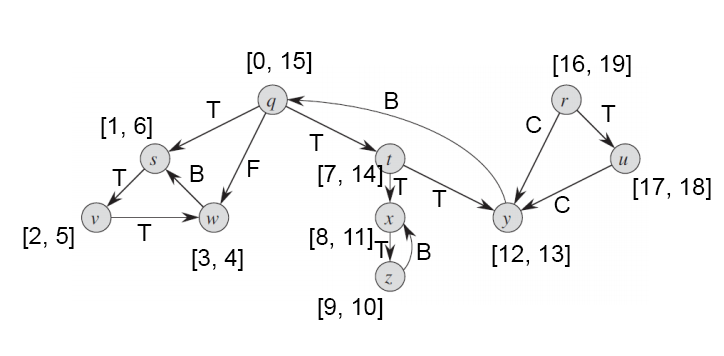
\includegraphics[width=\textwidth]{graph1}
T: Tree edge

B: Back edge

F: Forward edge

C: Cross edge

\section{DFS + BFS}
If BFS and DFS on a graph $G$ both return $T$, then $G$ must equal $T$. This is
true because the only time that BFS and DFS both return the same graph is when
$G$ consists solely of tree edges.

If there were any cross edge $e = (n, n')$ in $G$ after running BFS, then in 
DFS $n'$ would have become a direct child of $n$, and $T_{BFS} \neq T_{DFS} \neq G$.

If there were any forward edge $e = (n, n')$ in $G$ after running DFS, then in 
BFS $n'$ would be a direct child of $n$, and $T_{BFS} \neq T_{DFS} \neq G$.

If there were any back edge $e = (n, n')$ in $G$ after running DFS, then in
BFS $n'$ would be a direct child of $n$, and $T_{BFS} \neq T_{DFS} \neq G$.

\section{}
\subsection{i.}
The needed graph $G$ would be a graph containing all of the values $(x, y, z)$ 
with $x$ being the amount of water in the 10-pint jug, $y$ the amount in the 
7-pint jug, and $z$ the amount in the 4-pint jug, i.e.
$x \leq 10, y \leq 7, z \leq 4$. The edges of $G$ would be the valid transitions
in the puzzle between all possible valid puzzle states. A valid transition
is a valid move according to the rules of the puzzle, specifically, that in any
given move exactly one jug must be emptied or one must be filled, and the total
volume of water must be 11.

To solve the puzzle, we must determine if there is a path $p$ from $(0, 7, 4)$
to $(x, 2, z)$ or $(x, y, 2)$.

\subsection{ii.}
Using this configuration, a DFS on $G$ should determine whether such a path 
exists. 

\subsection{iii.}
DFS by following valid edges with the greatest $x$, then $y$, then $z$ values.
\begin{verbatim}
	(0, 7, 4)
	Out edges: (7, 0, 4), (4, 7, 0)
	(7, 0, 4)
	Out edges: (0, 7, 4), (7, 4, 0), (10, 0, 1)
	(10, 0, 1)
	Out edges: (3, 7, 1), (7, 0, 4), (10, 1, 0)
	(10, 1, 0)
	Out edges: (6, 1, 4), (10, 0, 1), (4, 7, 0)
	Already saw (10, 0, 1)
	(6, 1, 4)
	Out edges: (0, 7, 4), (10, 1, 0), (6, 5, 0)
	Already saw (10, 1, 0)
	(6, 5, 0)
	Out edges: (2, 5, 4), (4, 7, 0), (6, 1, 4)
	Already saw (6, 1, 4)
	(4, 7, 0)
	Out edges: (0, 7, 4), (10, 1, 0), (4, 3, 4)
	Already saw (10, 1, 0)
	(4, 3, 4)
	Out edges: (7, 0, 4), (8, 3, 0), (0, 7, 4)
	Already saw (7, 0, 4)
	(8, 3, 0)
	Out edges: (10, 1, 0), (4, 3, 4), (4, 7, 0)
	Already saw (10, 1, 0), (4, 3, 4), (4, 7, 0)
	Back to (4, 3, 4)
	Already saw (8, 3, 0), (0, 7, 4)
	Back to (4, 7, 0)
	Already saw (0, 7, 4), (4, 3, 4)
	Back to (6, 5, 0)
	Already saw (4, 7, 0), (6, 1, 4)
	(2, 5, 4)
	Out edges: (2, 7, 2), (6, 5, 0), (0, 7, 4)
	Already saw (6, 5, 0)
	(2, 7, 2)
\end{verbatim}
The result is $(0, 7, 4) \rightarrow (7, 0, 4) \rightarrow (10, 0, 1) 
\rightarrow (10, 1, 0) \rightarrow (6, 1, 4) \rightarrow (6, 5, 0)
\rightarrow (2, 5, 4) \rightarrow (2, 7, 2)$

\section{}
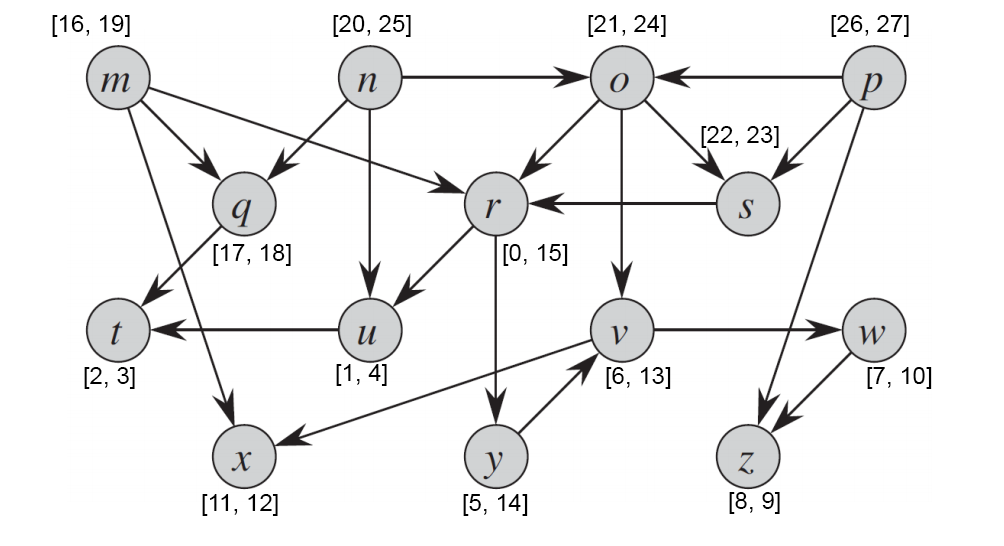
\includegraphics[width=\textwidth]{graph2}
Exit times: $27, 25, 24, 23, 19, 18, 15, 14, 13, 12, 10, 9, 4, 3$

Topological order: $p, n, o, s, m, q, r, y, v, x, w, z, u, t$

\section{Connectivity}
\subsection{i.}
Doing BFS on $G$ from node $u$ produces tree $T$ containing every vertex in $G$
with exactly one path $u \leadsto v'\ \forall \ v' \in T$. Removing any vertex 
$v \in T$ with no descendants ensures that $T$ remains connected, which means 
that $G$ is still connected.

\subsection{ii.}
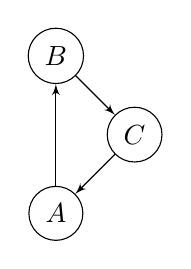
\begin{tikzpicture}
	\tikzset{vertex/.style = {shape=circle, draw, minimum size=1.5em}}
	\tikzset{edge/.style = {->, > = latex'}}
	\node[vertex] (a) at (0, 0) {$A$};
	\node[vertex] (b) at (0, 2) {$B$};
	\node[vertex] (c) at (1, 1) {$C$};
	\draw[edge] (a) to (b);
	\draw[edge] (b) to (c);
	\draw[edge] (c) to (a);
\end{tikzpicture}

\subsection{iii.}
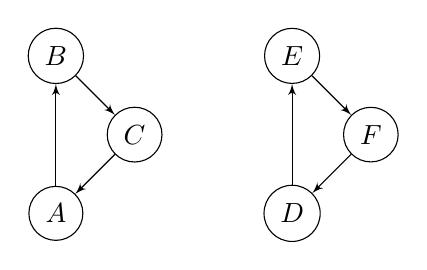
\begin{tikzpicture}
	\tikzset{vertex/.style = {shape=circle, draw, minimum size=1.5em}}
	\tikzset{edge/.style = {->, > = latex'}}
	\node[vertex] (a) at (0, 0) {$A$};
	\node[vertex] (b) at (0, 2) {$B$};
	\node[vertex] (c) at (1, 1) {$C$};
	\node[vertex] (d) at (3, 0) {$D$};
	\node[vertex] (e) at (3, 2) {$E$};
	\node[vertex] (f) at (4, 1) {$F$};
	\draw[edge] (a) to (b);
	\draw[edge] (b) to (c);
	\draw[edge] (c) to (a);
	\draw[edge] (d) to (e);
	\draw[edge] (e) to (f);
	\draw[edge] (f) to (d);
\end{tikzpicture}

\section{}
\subsection{i.}
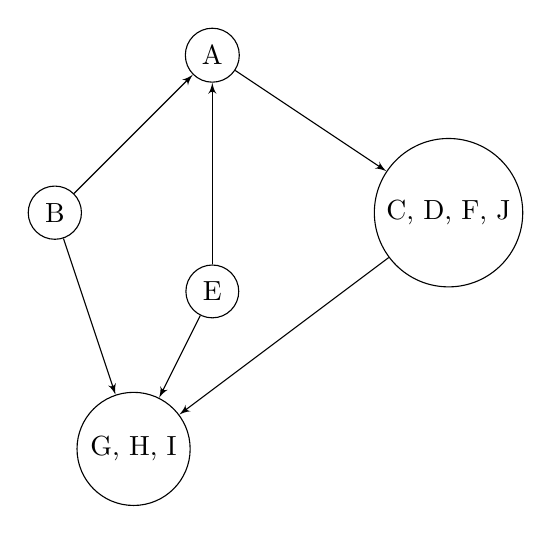
\begin{tikzpicture}
	\tikzset{vertex/.style = {shape=circle, draw, minimum size=1.5em}}
	\tikzset{edge/.style = {->, > = latex'}}
	\node[vertex] (ghi) at (1, 0) {G, H, I};
	\node[vertex] (cdfj) at (5, 3) {C, D, F, J};
	\node[vertex] (a) at (2, 5) {A};
	\node[vertex] (b) at (0, 3) {B};
	\node[vertex] (e) at (2, 2) {E};
	\draw[edge] (b) to (a);
	\draw[edge] (e) to (a);
	\draw[edge] (b) to (ghi);
	\draw[edge] (e) to (ghi);
	\draw[edge] (a) to (cdfj);
	\draw[edge] (cdfj) to (ghi);
\end{tikzpicture}

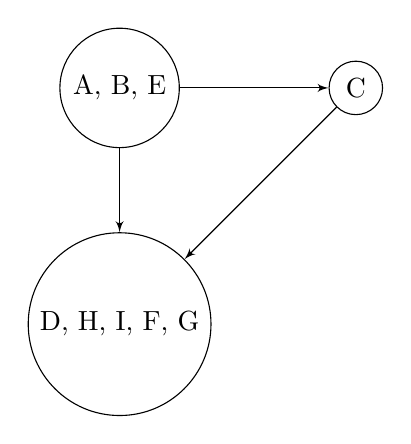
\begin{tikzpicture}
	\tikzset{vertex/.style = {shape=circle, draw, minimum size=1.5em}}
	\tikzset{edge/.style = {->, > = latex'}}
	\node[vertex] (abe) at (0, 3) {A, B, E};
	\node[vertex] (dhifg) at (0, 0) {D, H, I, F, G};
	\node[vertex] (c) at (3, 3) {C};
	\draw[edge] (abe) to (c);
	\draw[edge] (c) to (dhifg);
	\draw[edge] (abe) to (dhifg);
\end{tikzpicture}

\subsection{ii.}
E, B, A, (G, H, I), (C, J, F, D)

(A, E, B), C, (F, H, I, D, G)

\section{}
\begin{algorithm}
	\caption{Explore every vertex connected to $v$ in graph $G$ and set their 
		discover and exit times}
	\begin{lstlisting}[language=Python]
def explore(G, v):
	counter = 0
	stack = Stack()
	stack.put_on_top(v)

	while stack.is_not_empty():
		current = stack.peek_top()
		if not current.visited:
			# set current.visited, set discovery time, and increment counter
			pre_visit(counter, current)
			
			for w in current.reachable:
				if not w.visited 
				and not stack.contains(w):
					stack.put_on_top(w)

		else:
			# set exit time, and increment counter
			post_visit(counter, current)
			stack.pop_top()
	\end{lstlisting}
\end{algorithm}


\end{document}
